\documentclass[journal]{IEEEtran}
\usepackage[a5paper, margin=10mm, onecolumn]{geometry}
\usepackage{tfrupee}

\setlength{\headheight}{1cm}
\setlength{\headsep}{0mm}

\usepackage{cite}
\usepackage{amsmath,amssymb,amsfonts,amsthm}
\usepackage{algorithmic}
\usepackage{graphicx}
\usepackage{textcomp}
\usepackage{xcolor}
\usepackage{listings}
\usepackage{enumitem}
\usepackage{mathtools}
\usepackage{gensymb}
\usepackage{comment}
\usepackage[breaklinks=true]{hyperref}
\usepackage{tkz-euclide}
\usepackage{longtable}
\usepackage{multirow}
\usepackage{hhline}
\usepackage{array}

\begin{document}

\bibliographystyle{IEEEtran}
\vspace{3cm}

\title{4.2.1.1}
\author{EE24BTECH11004 - Ankit Jainar}
\maketitle

\renewcommand{\thefigure}{\theenumi}
\renewcommand{\thetable}{\theenumi}
\setlength{\intextsep}{10pt}

\numberwithin{equation}{enumi}
\numberwithin{figure}{enumi}

\textbf{Question}
Find the roots of quadratic equation:\\
\begin{align}
    x^2 - 3x - 10 = 0
\end{align}

\section*{Solution}
The given equation can be solved using analytical and numerical methods. Let us explore both approaches.

\subsection*{ Quadratic Formula}
The standard quadratic equation is:
\begin{align}
    ax^2 + bx + c = 0
\end{align}
Here, \( a = 1, b = -3, c = -10 \). The roots are given by:
\begin{align}
    x = \frac{-b \pm \sqrt{b^2 - 4ac}}{2a}
\end{align}
Substitute the values of \( a, b, \) and \( c \):
\begin{align}
    x = \frac{-(-3) \pm \sqrt{(-3)^2 - 4(1)(-10)}}{2(1)} \\
    x = \frac{3 \pm \sqrt{9 + 40}}{2} \\
    x = \frac{3 \pm \sqrt{49}}{2}
\end{align}
Simplify further:
\begin{align}
    x_1 = \frac{3 + 7}{2} = 5, \quad x_2 = \frac{3 - 7}{2} = -2
\end{align}

Thus, the roots of the equation are:
\begin{align}
    x_1 = 5, \quad x_2 = -2
\end{align}
\subsection*{ Solution using Matrix Approach by finding eigen values}
\subsection*{Matrix-Based Method}
For a polynomial equation of the form:
\begin{align}
    x^n + b_{n-1}x^{n-1} + \cdots + b_2x^2 + b_1x + b_0 = 0
\end{align}
we construct a matrix called the \textit{companion matrix}, which is defined as:
\begin{align}
    \Lambda =
    \begin{bmatrix}
        0 & 1 & 0 & \cdots & 0 \\
        0 & 0 & 1 & \cdots & 0 \\
        \vdots & \vdots & \vdots & \ddots & \vdots \\
        0 & 0 & 0 & \cdots & 1 \\
        -b_0 & -b_1 & -b_2 & \cdots & -b_{n-1}
    \end{bmatrix}
\end{align}

The eigenvalues of this matrix are the roots of the given polynomial equation.

For the quadratic equation \( x^2 - 3x - 10 = 0 \), we can write it as:
\begin{align}
    x^2 + (-3)x + (-10) = 0
\end{align}
The coefficients are:
\begin{align*}
    b_1 = -3, \quad b_0 = -10
\end{align*}

The companion matrix for this equation is:
\begin{align}
    \Lambda =
    \begin{bmatrix}
        0 & 1 \\
        -(-10) & -(-3)
    \end{bmatrix}
    =
    \begin{bmatrix}
        0 & 1 \\
        10 & 3
    \end{bmatrix}
\end{align}

\subsection*{Eigenvalue Computation}
The eigenvalues of \( \Lambda \) are obtained by solving:
\begin{align}
    \det(\Lambda - \lambda I) = 0
\end{align}
Substitute \( \Lambda \):
\begin{align}
    \begin{vmatrix}
        0 - \lambda & 1 \\
        10 & 3 - \lambda
    \end{vmatrix}
    = 0
\end{align}
Simplify the determinant:
\begin{align}
    (-\lambda)(3 - \lambda) - (10)(1) = 0 \\
    \lambda^2 - 3\lambda - 10 = 0
\end{align}

This is the original quadratic equation, so the eigenvalues are:
\begin{align}
    \lambda_1 = 5, \quad \lambda_2 = -2
\end{align}
\section*{QR Algorithm for Finding Eigenvalues and Roots of a Quadratic Equation}

Consider the quadratic equation:
\[
x^2 - 3x - 10 = 0
\]
We aim to find its roots using the QR algorithm, which finds the eigenvalues of the companion matrix of the quadratic polynomial.

\subsection*{1. Companion Matrix of the Polynomial}
The companion matrix \( \Lambda \) of the polynomial \( x^2 - 3x - 10 \) is given by:
\[
\Lambda = \begin{pmatrix} 
0 & 1 \\
-\frac{10}{1} & \frac{-3}{1}
\end{pmatrix}
= \begin{pmatrix}
0 & 1 \\
-10 & -3
\end{pmatrix}
\]
This matrix represents the system that corresponds to the given polynomial.

\subsection*{2. QR Decomposition}
The QR algorithm starts by performing QR decomposition on the matrix \( \Lambda \). The goal is to decompose \( \Lambda \) into an orthogonal matrix \( Q \) and an upper triangular matrix \( R \), such that:
\[
\Lambda = QR
\]
where \( Q^T Q = I \), and \( R \) is upper triangular. Then, we form a new matrix \( \Lambda' \) as:
\[
\Lambda' = RQ
\]
This process is repeated iteratively until \( \Lambda' \) converges to an upper triangular matrix whose diagonal elements are the eigenvalues of \( \Lambda \), which correspond to the roots of the quadratic equation.

\subsection*{3. Iterative Process}
Let’s outline the iterative steps for the QR algorithm applied to this companion matrix.

\subsubsection*{First Iteration:}
We start with \( \Lambda_0 = \begin{pmatrix} 0 & 1 \\ -10 & -3 \end{pmatrix} \).

Perform the QR decomposition of \( \Lambda_0 \):
\[
\Lambda_0 = QR
\]
Let’s calculate \( Q \) and \( R \), then form \( \Lambda_1 = RQ \).

\subsubsection*{Subsequent Iterations:}
Repeat the QR decomposition on the new matrix \( \Lambda_1 \), then form \( \Lambda_2 = RQ \), and so on, until the matrix \( \Lambda_k \) converges to an upper triangular form. The diagonal elements of this matrix represent the eigenvalues of \( \Lambda_0 \), which are the roots of the quadratic equation.

\subsection*{4. Eigenvalues and Roots}
After sufficient iterations, the QR algorithm will converge to an upper triangular matrix where the diagonal entries are the eigenvalues. These eigenvalues correspond to the roots of the polynomial. In this case, the eigenvalues of the companion matrix \( \Lambda \) will give us the roots of the quadratic equation \( x^2 - 3x - 10 = 0 \).

Thus, the eigenvalues (roots) are the solutions to the quadratic equation:
\[
x = \frac{3 \pm \sqrt{3^2 - 4(1)(-10)}}{2(1)} = \frac{3 \pm \sqrt{9 + 40}}{2} = \frac{3 \pm \sqrt{49}}{2}
\]
\[
x = \frac{3 \pm 7}{2}
\]
Hence, the roots are:
\[
x_1 = 5, \quad x_2 = -2
\]

\subsection*{ Solution using Fixed Point Iteration}
We rewrite the equation as:
\begin{align}
    x = g(x)
\end{align}
A possible choice for \( g(x) \) is:
\begin{align}
    g(x) = \sqrt{3x + 10}
\end{align}
The iterative update becomes:
\begin{align}
    x_{n+1} = \sqrt{3x_n + 10}
\end{align}

Starting with an initial guess \( x_0 = 2 \), the iterations are as follows:
\begin{align}
    x_1 = \sqrt{3(2) + 10} = \sqrt{16} = 4 \\
    x_2 = \sqrt{3(4) + 10} = \sqrt{22} \approx 4.69 \\
    x_3 = \sqrt{3(4.69) + 10} \approx 5.14 \\
    \vdots
\end{align}
\textbf{Observation:} The iterations converge to \( x = 5 \), one of the roots of the quation. For \( x_2 = -2 \), a similar setup with \( g(x) = -\sqrt{3x + 10} \) would be used.

\subsection*{ Newton-Raphson Method}
The Newton-Raphson method is defined as:
\begin{align}
    x_{n+1} = x_n - \frac{f(x_n)}{f'(x_n)}
\end{align}
Here:
\begin{align}
    f(x) = x^2 - 3x - 10, \quad f'(x) = 2x - 3
\end{align}
Substitute into the formula:
\begin{align}
    x_{n+1} = x_n - \frac{x_n^2 - 3x_n - 10}{2x_n - 3}
\end{align}

\textbf{Example: Starting with an initial guess \( x_0 = 3 \):}
\begin{align}
    x_1 = 3 - \frac{3^2 - 3(3) - 10}{2(3) - 3} = 3 - \frac{9 - 9 - 10}{6 - 3} = 3 + \frac{10}{3} \approx 6.33 \\
    x_2 = 6.33 - \frac{6.33^2 - 3(6.33) - 10}{2(6.33) - 3} \approx 5.02
\end{align}
\textbf{Observation:} The iterations quickly converge to \( x = 5 \). Similarly, starting with \( x_0 = -1 \) converges to \( x = -2 \).

\section*{Computational Approach}
The following results were obtained using a computational method:
\begin{align*}
\text{Running Fixed Point Iterations Method:} 
\text{Root 1:} & \; 5 \\
\text{Root 2:} & \; -2 \\
\text{Running Newton-Raphson Method:} & \\
\text{Root 1:} & \; 5 \\
\text{Root 2:} & \; -2
\end{align*}


\section*{Conclusion}
The roots of the quadratic equation \( x^2 - 3x - 10 = 0 \) are:
\begin{align}
    x_1 = 5, \quad x_2 = -2
\end{align}
Both numerical and analytical methods confirm these results.
Here are the roots of the Quadratic Equation 
\begin{align}
    x^2 - 3x - 10 = 0
\end{align} in plotted below.\\

\begin{figure}[h!]
   \centering
   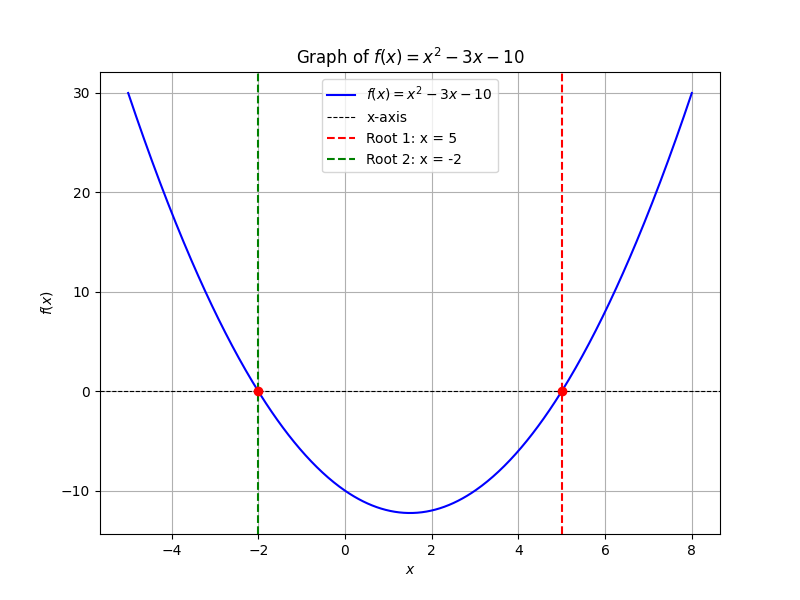
\includegraphics[width=0.7\columnwidth]{figs/fig.png}
\end{figure}

\end{document}
